\documentclass[a4paper,14pt]{article}

\usepackage{pgfpages}

\usepackage[T2A]{fontenc}
\usepackage[utf8]{inputenc}
\usepackage[russian]{babel}

\usepackage{physics}
\usepackage{amsthm, amsmath, amssymb}
\usepackage{mathtext}
\usepackage[makeroom]{cancel}

% biber recommends this
\usepackage{csquotes}

\usepackage[
    colorlinks=true,
    linkcolor=black,
    anchorcolor=black,
    citecolor=black,
    filecolor=black,
    menucolor=black,
    runcolor=black,
    urlcolor=black
]{hyperref}
\usepackage[backend=biber,citestyle=numeric]{biblatex}
\addbibresource{~/data/references.bib}

\usepackage{graphicx}
\usepackage{graphbox}
\graphicspath{ {./images/} }

\linespread{1.5}
\setlength{\parindent}{1.25cm}

\usepackage{geometry}
\geometry{left=3cm}
\geometry{right=1.5cm}
\geometry{top=2cm}
\geometry{bottom=2cm}

\newtheorem{theorem}{Теорема}
% \newtheorem{proposition}{Утверждение}
\newtheorem{lemma}{Лемма}
\newtheorem{problem}{Задача}

\theoremstyle{definition}
\newtheorem{definition}{Определение}
\newtheorem{corollary}{Следствие}


\title{Оценка перерегулирования дифференциально-разностных управляемых систем}
\author{Шаршуков Владислав}
\date{2023}

\begin{document}

\begin{titlepage}
  \begin{center}
    САНКТ-ПЕТЕРБУРГСКИЙ ГОСУДАРСТВЕННЫЙ УНИВЕРСИТЕТ \\
    Направление: 01.03.02 «Прикладная математика и информатика» \\
    ООП: Прикладная математика, фундаментальная информатика и программирование \\[4cm]

    \textbf{ОТЧЕТ О НАУЧНО-ИССЛЕДОВАТЕЛЬСКОЙ РАБОТЕ}\\
  \end{center}
  \textbf{Тема задания:} Оценка перерегулирования
  дифференциально-разностных управляемых систем \\[0.5cm]
  \textbf{Выполнил:} Шаршуков Владислав \qquad 20.Б04-пу \\ [1.5cm]
  \textbf{Руководитель практики:} \\Жабко Алексей Петрович,
  доктор физ.-мат. наук, профессор, заведующий кафедрой теории
  управления
  \vspace{5cm}
  \begin{center}
    Санкт-Петербург\\
    2023
  \end{center}
\end{titlepage}

\setcounter{page}{2}

\begin{center}
  \tableofcontents
\end{center}

\newpage

\section{Введение}

\section{Обзор литературы}

Разные подходы: через решение матричных неравенств~\cite{modie2005},
через оценки функционала полного типа~\cite{kharitonov2013, kharitonov2004},

В настоящей работе рассматривается скалярное уравнение с постоянным
запаздыванием, для которого вариационными методами будет получена
точная оценка функционала полного типа.

\section{Постановка задачи}
Рассмотрим скалярное дифференциальное уравнение с запаздыванием:
\begin{equation}
  \label{eq:main-system}
  \dot x(t) = a_0 x(t) + a_1 x(t - h),
  \qquad h = \mathrm{const} > 0,
  \quad a_1 \neq 0.
\end{equation}
Будем считать систему~\eqref{eq:main-system} экспоненциально устойчивой.
В этом случае справедливо~\cite[стр.~66]{kharitonov2013}, что если
$U(\tau)$ --- матрица Ляпунова для матрицы $W = W_0 + W_1 + W_2 h$, причём
$W_0, W_1, W_2 > 0$, то функционал полного типа
\begin{equation}
  \label{eq:complete-type-functional}
  \begin{aligned}
    v(\varphi)
    &=
      U(0) \varphi^2(0)
      +
      2 a_1 \varphi(0) \int\limits_{-h}^{0} U(-h - \theta) \varphi(\theta) d\theta
      + \\
    &\phantom{=}
      +
      \int\limits_{-h}^{0} a_1^2 \varphi(\theta_1) \left[
      \int\limits_{-h}^{0} U(\theta_1 - \theta_2) \varphi(\theta_2) d\theta_2
      \right] d\theta_1
      + \\
    &\phantom{=}
      +
      \int\limits_{-h}^{0} \left[
      W_1 + (h + \theta) W_2
      \right] \varphi^2(\theta) d\theta
  \end{aligned}
\end{equation}
допускает оценку
\begin{equation}
  \label{eq:functional-estimation}
  \alpha_1 \norm{\varphi(0)}^2
  \leqslant
  v(\varphi)
  \leqslant
  \alpha_2 \norm{\varphi}_h^2,
  \qquad
  \varphi \in PC([-h, 0], \mathbb{R}),
\end{equation}
где $\alpha_1, \alpha_2 > 0$ --- некоторые константы. Решение исходной
системы~\eqref{eq:main-system} тогда~\cite[стр.~67]{kharitonov2013} допускает
оценку
\begin{equation*}
  \norm{x(t, \varphi)} \leqslant \gamma \norm{\varphi}_h e^{-\sigma t},
  \qquad t \geqslant 0,
\end{equation*}
где $\gamma = \sqrt{\dfrac{\alpha_2}{\alpha_1}}$.

Заметим, что $\alpha_1$ и $\alpha_2$ можно рассматривать как функции переменных
$W_0, W_1, W_2$, поэтому можно поставить оптимизационную задачу: найти
максимальное значение для $\alpha_1$ и минимальное значение для $\alpha_2$, при
которых оценка~\eqref{eq:functional-estimation} справедлива.

\section{Основной результат}

Известно~\cite[стр.~51]{kharitonov2013}, что если система~\eqref{eq:main-system}
удовлетворяет условию Ляпунова, т.е. если спектр этой системы
\begin{equation*}
  \Lambda = \left\{ s \in \mathbb{C}: s - a_0 - e^{-sh} a_1 = 0 \right\}
\end{equation*}
не содержит ни одного корня $s_0$ такого, чтобы и $-s_0$ принадлежал спектру
$\Lambda$, то для любой симметричной матрицы $W$ существует единственная матрица
Ляпунова $U(\tau)$. Очевидно, для любой экспоненциально устойчивой системы
условие Ляпунова выполняется. Тогда по данной матрице Ляпунова $U(\tau)$
можно построить функционал полного типа~\eqref{eq:complete-type-functional},
допускающий оценку~\eqref{eq:functional-estimation}.

\subsection{Вывод условий для нахождения $\alpha_1$}

Рассмотрим вспомогательный функционал
\begin{equation*}
  \begin{aligned}
    g_1(\varphi)
    &=
      v(\varphi) - \alpha_1 \norm{\varphi(0)}^2 = \\
    &=
      \left( U(0) - \alpha_1 \right) \varphi^2(0)
      +
      2 a_1 \varphi(0) \int\limits_{-h}^{0} U(-h - \theta) \varphi(\theta) d\theta
      + \\
    &\phantom{=}
      +
      \int\limits_{-h}^{0} a_1^2 \varphi(\theta_1) \left[
      \int\limits_{-h}^{0} U(\theta_1 - \theta_2) \varphi(\theta_2) d\theta_2
      \right] d\theta_1
      + \\
    &\phantom{=}
      +
      \int\limits_{-h}^{0} \left[
      W_1 + (h + \theta) W_2
      \right] \varphi^2(\theta) d\theta.
  \end{aligned}
\end{equation*}
Из оценки~\eqref{eq:functional-estimation} следует, что $g_1(\varphi) \geqslant 0$.
Понятно, что в случае тривиальной функции $\varphi(t) \equiv 0, \; t \in [-h, 0]$
функционал достигает своего минимума: $g_1(\varphi) = 0$. Однако в этом случае
оценка~\eqref{eq:functional-estimation} выполняется для любых $\alpha_1, \alpha_2$.
Выясним, при каких нетривиальных функциях $\varphi(t)$ и соответствующих им значениях
$\alpha_1$ у функционала $g_1(\varphi)$ найдутся точки, подозрительные на экстремум.

Необходимым условием экстремума функционала $g_1(\varphi)$ является условие равенства
нулю его первой вариации~\cite[стр.~19]{gelfand1961}:
\begin{equation}
  \label{eq:necessary-cond}
  \delta g_1(\varphi) = 0.
\end{equation}
Для её вычисления воспользуемся следующим определением~\cite[стр.~289]{elsgolc1969}:
\begin{equation}
  \label{eq:variation-def}
  \delta g_1(\varphi) = \left.
    \frac{\partial}{\partial \alpha} g_1(\varphi + \alpha \delta \varphi)
  \right|_{\alpha = 0}.
\end{equation}
Введём вспомогательные обозначения:
\begin{equation*}
  \begin{aligned}
    P_1(\varphi)
    &=
      2 a_1 \varphi(0) \int\limits_{-h}^{0} U(-h - \theta) \varphi(\theta) d\theta, \\
    P_2(\varphi)
    &=
      \int\limits_{-h}^{0} a_1^2 \varphi(\theta_1) \left[
      \int\limits_{-h}^{0} U(\theta_1 - \theta_2) \varphi(\theta_2) d\theta_2
      \right] d\theta_1.
  \end{aligned}
\end{equation*}
Прежде всего, пользуясь свойством симметричности матрицы Ляпунова~\cite[стр.~38]{kharitonov2013}
\begin{equation}
  \label{eq:lyapunov-symmetric-property}
  U(-\tau) = U^T(\tau), \qquad \tau \geqslant 0,
\end{equation}
перепишем выражение для $P_1(\varphi)$ в виде
\begin{equation*}
  P_1(\varphi)
  =
  2 a_1 \varphi(0) \int\limits_{-h}^{0} U(\theta + h) \varphi(\theta) d\theta.
\end{equation*}
Вычислим теперь первую вариацию $\delta P_1(\varphi)$ этого функционала. Пользуясь
определением~\eqref{eq:variation-def}, последовательно получаем
\begin{equation*}
  \begin{aligned}
    P_1(\varphi + \alpha \varphi)
    &=
      2 a_1 (\varphi(0) + \alpha \delta\varphi(0))
      \int\limits_{-h}^{0} U(\theta + h) (\varphi(\theta) + \alpha \delta\varphi(\theta)) d\theta,
    \\
    \frac{\partial }{\partial \alpha}
    P_1(\varphi + \alpha \varphi)
    &=
      2 a_1 \delta\varphi(0)
      \int\limits_{-h}^{0} U(\theta + h) (\varphi(\theta) + \alpha \delta\varphi(\theta)) d\theta
      +
      2 a_1 (\varphi(0) + \alpha \delta\varphi(0))
      \int\limits_{-h}^{0} U(\theta + h) \delta\varphi(\theta) d\theta,
    \\
    \delta P_1(\varphi)
    &=
      2 a_1 \delta\varphi(0)
      \int\limits_{-h}^{0} U(\theta + h) \varphi(\theta) d\theta
      +
      2 a_1 \varphi(0)
      \int\limits_{-h}^{0} U(\theta + h) \delta\varphi(\theta) d\theta.
  \end{aligned}
\end{equation*}
Аналогичным образом вычислим $\delta P_2(\varphi)$:
\begin{equation*}
  \begin{aligned}
    P_2(\varphi + \alpha \varphi)
    &=
      \int\limits_{-h}^{0} a_1^2 (\varphi(\theta_1) + \alpha \delta \varphi(\theta_1))
      \left[
      \int\limits_{-h}^{0}
      U(\theta_1 - \theta_2) (\varphi(\theta_2) + \alpha \delta \varphi(\theta_2))
      d\theta_2
      \right]
      d\theta_1
    \\
    \frac{\partial }{\partial \alpha}
    P_2(\varphi + \alpha \varphi)
    &=
      \int\limits_{-h}^{0} a_1^2 \delta \varphi(\theta_1)
      \left[
      \int\limits_{-h}^{0}
      U(\theta_1 - \theta_2) (\varphi(\theta_2) + \alpha \delta \varphi(\theta_2))
      d\theta_2
      \right]
      d\theta_1
      + \\
    &\phantom{=}
      +
      \int\limits_{-h}^{0} a_1^2 (\varphi(\theta_1) + \alpha \delta \varphi(\theta_1))
      \left[
      \int\limits_{-h}^{0}
      U(\theta_1 - \theta_2) \delta \varphi(\theta_2)
      d\theta_2
      \right]
      d\theta_1
    \\
    \delta P_2(\varphi)
    &=
      \int\limits_{-h}^{0} a_1^2 \delta \varphi(\theta_1)
      \left[
      \int\limits_{-h}^{0}
      U(\theta_1 - \theta_2) \varphi(\theta_2)
      d\theta_2
      \right]
      d\theta_1
      + \\
    &\phantom{=}
      +
      \int\limits_{-h}^{0} a_1^2 \varphi(\theta_1)
      \left[
      \int\limits_{-h}^{0}
      U(\theta_1 - \theta_2) \delta \varphi(\theta_2)
      d\theta_2
      \right]
      d\theta_1.
  \end{aligned}
\end{equation*}

Для последующих упрощений нам потребуется следующая
\begin{lemma}\label{lemma:symmetric-functional}
  Функционал
  \begin{equation}
    \label{eq:lemma-1-functional}
    h(\varphi, \psi)
    =
    \int\limits_{-h}^{0} \varphi(\theta_1)
    \left[
      \int\limits_{-h}^{0} U(\theta_2 - \theta_1) \psi(\theta_2) d\theta_2
    \right]
    d\theta_1
  \end{equation}
  симметричен, то есть $h(\varphi, \psi) = h(\psi, \varphi)$.
\end{lemma}

\begin{proof}
  Запишем функционал $h(\varphi, \psi)$ в виде
  \begin{equation*}
    h(\varphi, \psi)
    =
    \int\limits_{-h}^{0}
    \int\limits_{-h}^{0} U(\theta_2 - \theta_1) \varphi(\theta_1) \psi(\theta_2)
    d\theta_1
    d\theta_2.
  \end{equation*}
  Так как пределы интегрирования не зависят от $\theta_1$ и $\theta_2$, то порядок
  интегрирования можно поменять:
  \begin{equation*}
    h(\varphi, \psi)
    =
    \int\limits_{-h}^{0} \psi(\theta_2)
    \left[
      \int\limits_{-h}^{0} U(\theta_2 - \theta_1) \varphi(\theta_1) d\theta_1
    \right]
    d\theta_2.
  \end{equation*}
  Заменим теперь $\theta_1$ на $\theta_2$, а $\theta_2$ --- на $\theta_1$:
  \begin{equation*}
    h(\varphi, \psi)
    =
    \int\limits_{-h}^{0} \psi(\theta_1)
    \left[
      \int\limits_{-h}^{0} U(\theta_1 - \theta_2) \varphi(\theta_2) d\theta_2
    \right]
    d\theta_1.
  \end{equation*}
  Воспользуемся теперь свойством симметричности матрицы
  Ляпунова~\eqref{eq:lyapunov-symmetric-property}:
  \begin{equation*}
    \begin{aligned}
      h(\varphi, \psi)
      &=
        \int\limits_{-h}^{0} \psi(\theta_1)
        \left[
        \int\limits_{-h}^{0} U(\theta_1 - \theta_2) \varphi(\theta_2) d\theta_2
        \right]
        d\theta_1 = \\
      &=
        \int\limits_{-h}^{0} \psi(\theta_1)
        \left[
        \int\limits_{-h}^{0} U(\theta_2 - \theta_1) \varphi(\theta_2) d\theta_2
        \right]
        d\theta_1.
    \end{aligned}
  \end{equation*}
  Сравнивая правую часть полученного равенства с определением
  функционала~\eqref{eq:lemma-1-functional}, окончательно приходим
  к выводу, что
  \begin{equation*}
    h(\varphi, \psi) = h(\psi, \varphi).
  \end{equation*}
\end{proof}
Пользуясь леммой~\ref{lemma:symmetric-functional}, первую вариацию функционала $P_2(\varphi)$
можно записать как
\begin{equation*}
  \delta P_2(\varphi)
  =
  2
  \int\limits_{-h}^{0} a_1^2 \delta \varphi(\theta_1)
  \left[
    \int\limits_{-h}^{0}
    U(\theta_1 - \theta_2) \varphi(\theta_2)
    d\theta_2
  \right]
  d\theta_1.
\end{equation*}
Итак, окончательно получаем выражение для первой вариации функционала $g_1(\varphi)$:
\begin{equation*}
  \begin{aligned}
    \delta g_1(\varphi)
    &=
      2 \left( U(0) - \alpha_1 \right) \varphi(0) \delta \varphi(0)
      + \\
    &\phantom{=}
      +
      2 a_1 \delta\varphi(0)
      \int\limits_{-h}^{0} U(\theta + h) \varphi(\theta) d\theta
      +
      2 a_1 \varphi(0)
      \int\limits_{-h}^{0} U(\theta + h) \delta\varphi(\theta) d\theta
      + \\
    &\phantom{=}
      +
      2
      \int\limits_{-h}^{0} a_1^2 \delta \varphi(\theta_1)
      \left[
      \int\limits_{-h}^{0}
      U(\theta_1 - \theta_2) \varphi(\theta_2)
      d\theta_2
      \right]
      d\theta_1
      + \\
    &\phantom{=}
      +
      2 \int\limits_{-h}^{0}
      \left[ W_1 + (h + \theta) W_2 \right] \varphi(\theta) \delta \varphi(\theta)
      d\theta.
  \end{aligned}
\end{equation*}
Соберём слагаемые при одинаковых вариациях функции $\varphi$:
\begin{equation*}
  \begin{aligned}
    \delta g_1(\varphi)
    &=
      2
      \left[
      \left( U(0) - \alpha_1 \right) \varphi(0)
      +
      a_1
      \int\limits_{-h}^{0} U(\theta + h) \varphi(\theta) d\theta
      \right] \delta \varphi(0)
      + \\
    &\phantom{=}
      +
      2
      \int\limits_{-h}^{0}
      \left[
      a_1 \varphi(0)
      U(\theta + h)
      +
      a_1^2
      \int\limits_{-h}^{0}
      U(\theta - \theta_2) \varphi(\theta_2)
      d\theta_2
      +
      \left[ W_1 + (h + \theta) W_2 \right] \varphi(\theta)
      \right]
      \delta \varphi(\theta)
      d\theta.
  \end{aligned}
\end{equation*}
Рассмотрим сначала ситуацию, когда вариация функции $\varphi$ на конце
рассматриваемого промежутка равна нулю, то есть $\delta \varphi(0) = 0$.
Тогда из необходимого условия экстремума функционала~\eqref{eq:necessary-cond}
следует, что
\begin{equation*}
  \int\limits_{-h}^{0}
  \left[
    a_1 \varphi(0)
    U(\theta + h)
    +
    a_1^2
    \int\limits_{-h}^{0}
    U(\theta - \theta_2) \varphi(\theta_2)
    d\theta_2
    +
    \left[ W_1 + (h + \theta) W_2 \right] \varphi(\theta)
  \right]
  \delta \varphi(\theta)
  d\theta
  = 0.
\end{equation*}
В силу произвольности вариации $\delta \varphi$ из основной леммы
вариационного исчисления~\cite[стр.~295]{elsgolc1969} следует,
что
\begin{equation*}
  a_1 \varphi(0)
  U(\theta + h)
  +
  a_1^2
  \int\limits_{-h}^{0}
  U(\theta - \theta_2) \varphi(\theta_2)
  d\theta_2
  +
  \left[ W_1 + (h + \theta) W_2 \right] \varphi(\theta)
  = 0.
\end{equation*}

Пусть теперь $\delta \varphi(0) \neq 0$. Тогда из необходимого условия
экстремума функционала~\eqref{eq:necessary-cond} следует, что
\begin{equation*}
  \left[
    \left( U(0) - \alpha_1 \right) \varphi(0)
    +
    a_1
    \int\limits_{-h}^{0} U(\theta + h) \varphi(\theta) d\theta
  \right] \delta \varphi(0)
  = 0,
\end{equation*}
откуда в силу произвольности вариации $\delta \varphi(0)$
следует, что
\begin{equation*}
  \left( U(0) - \alpha_1 \right) \varphi(0)
  +
  a_1
  \int\limits_{-h}^{0} U(\theta + h) \varphi(\theta) d\theta
  = 0.
\end{equation*}

Итак, объединяя полученные результаты, получаем необходимые условия
экстремума функционала $g_1(\varphi)$:
\begin{align}
  \label{eq:necessary-cond-for-g1-1}
  a_1 \varphi(0)
  U(\theta + h)
  +
  a_1^2
  \int\limits_{-h}^{0}
  U(\theta - \theta_2) \varphi(\theta_2)
  d\theta_2
  +
  \left[ W_1 + (h + \theta) W_2 \right] \varphi(\theta)
  = 0, \\
  \label{eq:necessary-cond-for-g1-2}
  \left( U(0) - \alpha_1 \right) \varphi(0)
  +
  a_1
  \int\limits_{-h}^{0} U(\theta + h) \varphi(\theta) d\theta
  = 0.
\end{align}
Рассмотрим уравнение~\eqref{eq:necessary-cond-for-g1-1}. Так как
$W_1, W_2 > 0$, а $\theta \in [-h, 0]$, то
\begin{equation*}
  W_1 + (h + \theta) W_2 > 0,
\end{equation*}
поэтому можно разделить обе части этого уравнения на эту величину:
\begin{equation*}
    a_1 \varphi(0)
    U(\theta + h)
    \frac{1}{W_1 + (\theta + h) W_2}
    +
    a_1^2
    \frac{1}{W_1 + (\theta + h) W_2}
    \int\limits_{-h}^{0}
    U(\theta - \theta_2) \varphi(\theta_2)
    d\theta_2
    +
    \varphi(\theta)
    = 0.
\end{equation*}
Введём обозначения:
\begin{equation}
  \label{eq:necessary-cond-notation}
  \begin{aligned}
    K_1(\theta, t)
    &=
      \frac{U(\theta - t)}{W_1 + (\theta + h) W_2},
    &
      f_1(\theta)
    &=
      - a_1
      \frac{U(\theta + h)}{W_1 + (\theta + h) W_2},
    &
      \lambda &= -a_1^2, \\
    K_2(\theta, t)
    &=
      a_1 U(\theta + h),
    &
      f_2(\theta, \alpha_1)
    &=
      \alpha_1 - U(0)
  \end{aligned}
\end{equation}
Используя их, уравнения~\eqref{eq:necessary-cond-for-g1-1}
и~\eqref{eq:necessary-cond-for-g1-2} окончательно представляются
в виде
\begin{align}
  \label{eq:g1-fredholm-2}
  \varphi(\theta)
  &=
    \lambda
    \int\limits_{-h}^{0}
    K_1(\theta, t)
    \varphi(t)
    dt
    + f_1(\theta) \varphi(0), \\
  \label{eq:g1-fredholm-1}
  f_2(\theta, \alpha_1) \varphi(0)
  &=
    \int\limits_{-h}^{0}
    K_2(\theta, t)
    \varphi(t)
    dt.
\end{align}
Так как ядра $K_1(\theta, t)$ и $K_2(\theta, t)$ полученных интегральных
уравнений непрерывны в квадрате
\begin{equation*}
  S = \left\{ -h \leqslant \theta \leqslant 0, -h \leqslant t \leqslant 0 \right\},
\end{equation*}
то они являются фредгольмовыми~\cite[стр.~78]{manzhirov2000}, а сами
уравнения~\eqref{eq:g1-fredholm-2} и~\eqref{eq:g1-fredholm-2} представляют собой
интегральные уравнения Фредгольма 2-го и 1-го рода соответственно.

\subsection{Вывод условий для нахождения $\alpha_2$}

Рассмотрим вспомогательный функционал
\begin{equation*}
  g_2(\varphi)
  =
  v(\varphi) - \alpha_2 \norm{\varphi}_h^2.
\end{equation*}
Из оценки~\eqref{eq:functional-estimation} следует, что $g_2(\varphi) \leqslant 0$.
По аналогии с функционалом $g_1(\varphi)$ выясним, при каких нетривиальных функциях
$\varphi(t)$ и соответствующих им значениях $\alpha_2$ найдутся точки, подозрительные
на экстремум.

Рассмотрим выражение $g_2(\varphi + \alpha \delta \varphi)$. Пусть
\begin{equation*}
  \theta^*
  = \arg\sup_{\theta \in [-h, 0]} \abs{\varphi(\theta) + \alpha \delta \varphi(\theta)},
\end{equation*}
тогда
\begin{equation*}
  g_2(\varphi + \alpha \delta \varphi)
  = v(\varphi + \alpha \delta \varphi)
  - \alpha_2 {(\varphi(\theta^*) + \alpha \delta \varphi(\theta^*))}^2.
\end{equation*}
Заметим, что в частном случае точка $\theta^*$ может совпадать с точкой, в которой
достигается супремум функции $\abs{\varphi(\theta)}$.

Пользуясь выкладками, полученными в предыдущем пункте, запишем выражение для первой вариации
функционала $g_2(\varphi)$:
\begin{equation*}
  \begin{aligned}
    \delta g_2(\varphi)
    &=
      2
      \left[
      U(0) \varphi(0)
      +
      a_1
      \int\limits_{-h}^{0} U(\theta + h) \varphi(\theta) d\theta
      \right] \delta \varphi(0)
      -
      2 \alpha_2 \varphi(\theta^*) \delta \varphi(\theta^*)
      + \\
    &\phantom{=}
      +
      2
      \int\limits_{-h}^{0}
      \left[
      a_1 \varphi(0)
      U(\theta + h)
      +
      a_1^2
      \int\limits_{-h}^{0}
      U(\theta - \theta_2) \varphi(\theta_2)
      d\theta_2
      +
      \left[ W_1 + (h + \theta) W_2 \right] \varphi(\theta)
      \right]
      \delta \varphi(\theta)
      d\theta.
  \end{aligned}
\end{equation*}
Предположим, что $\theta^* \neq 0$, тогда из независимости вариаций следуют следующие
необходимые условия экстремума функционала $g_2(\varphi)$:
\begin{equation*}
  \begin{aligned}
  a_1 \varphi(0)
  U(\theta + h)
  +
  a_1^2
  \int\limits_{-h}^{0}
  U(\theta - \theta_2) \varphi(\theta_2)
  d\theta_2
  +
  \left[ W_1 + (h + \theta) W_2 \right] \varphi(\theta)
  = 0, \\
  U(0) \varphi(0)
  +
  a_1
  \int\limits_{-h}^{0} U(\theta + h) \varphi(\theta) d\theta
    = 0, \\
    \alpha_2 \varphi(\theta^*) = 0.
  \end{aligned}
\end{equation*}
Заметим, что $\varphi(\theta^*) \neq 0$, так как в противном случае из определения
точки $\theta^*$ следовало бы, что $\varphi(t) \equiv 0, t \in [-h, 0]$. Учитывая,
что $\alpha_2 > 0$, заключаем, что нетривиальные функции, для которых $\theta^* \neq 0$,
не являются экстремалями функционала $g_2(\varphi)$.

Рассмотрим теперь функции, для которых $\theta^* = 0$. В этом случае необходимые
условия экстремума функционала $g_2(\varphi)$ примут вид
\begin{equation*}
  \begin{aligned}
  a_1 \varphi(0)
  U(\theta + h)
  +
  a_1^2
  \int\limits_{-h}^{0}
  U(\theta - \theta_2) \varphi(\theta_2)
  d\theta_2
  +
  \left[ W_1 + (h + \theta) W_2 \right] \varphi(\theta)
  = 0, \\
  (U(0) - \alpha_2) \varphi(0)
  +
  a_1
  \int\limits_{-h}^{0} U(\theta + h) \varphi(\theta) d\theta
    = 0.
  \end{aligned}
\end{equation*}
Пользуясь обозначениями~\eqref{eq:necessary-cond-notation}, эти условия можно записать
в виде
\begin{equation*}
  \begin{aligned}
    \varphi(\theta)
    &=
      \lambda
      \int\limits_{-h}^{0}
      K_1(\theta, t)
      \varphi(t)
      dt
      + f_1(\theta) \varphi(0), \\
    f_2(\theta, \alpha_2) \varphi(0)
    &=
      \int\limits_{-h}^{0}
      K_2(\theta, t)
      \varphi(t)
      dt.
  \end{aligned}
\end{equation*}
Выходит, что вид условий для экстремалей функционала $g_2(\varphi)$ совпадает с условиями для
экстремалей функционала $g_1(\varphi)$. Заметим, что ключевое различие заключается
в том, что $g_1(\varphi) \geqslant 0$, а $g_2(\varphi) \leqslant 0$.

\subsection{Анализ множеств $\mathcal{A}_0$, $\mathcal{A}_+$ и $\mathcal{A}_-$}

Рассмотрим функционал
\begin{equation*}
  g(\varphi, \alpha) = v(\varphi) - \alpha \varphi^2(0).
\end{equation*}
Пусть $\mathbb{R}_+$ --- множество вещественных положительных чисел.
Обозначим через $\mathcal{F}_0 \subset PC([-h, 0], \mathbb{R})$ множество нетривиальных
кусочно-непрерывных функций, обращающих функционал $g(\varphi, \alpha)$ в ноль при некотором
$\alpha \in \mathbb{R}_+$. Множество таких $\alpha$ обозначим за $\mathcal{A}_0$, то есть
\begin{equation*}
  \mathcal{A}_0 = \left\{
    \alpha \in \mathbb{R}_+: \exists \varphi \in \mathcal{F}_0 \quad g(\varphi, \alpha) = 0
  \right\}.
\end{equation*}
Введём два дополнительных обозначения:
\begin{equation*}
  \begin{aligned}
    \mathcal{A}_+
    &=
      \left\{
      \alpha \in \mathbb{R}_+ :
      g(\varphi, \alpha) \geqslant 0 \quad \forall \varphi \in PC([-h, 0], \mathbb{R})
      \right\} \subset \mathbb{R}_+, \\
    \mathcal{A}_-
    &=
      \left\{
      \alpha \in \mathbb{R}_+ :
      g(\varphi, \alpha) \leqslant 0 \quad \forall \varphi \in PC([-h, 0], \mathbb{R})
      \right\} \subset \mathbb{R}_+.
  \end{aligned}
\end{equation*}
Заметим, что из существования оценки~\eqref{eq:functional-estimation} следует, что
множества $\mathcal{A}_+$ и $\mathcal{A}_-$ непусты.

\begin{lemma}
  Множества $\mathcal{A}_+$ и $\mathcal{A}_-$ выпуклы.
\end{lemma}

\begin{proof}
  Пусть $\alpha_1, \alpha_2 \in \mathcal{A}_+$, тогда для любой
  $\varphi \in PC([-h, 0], \mathbb{R})$ выполняются неравенства
  \begin{equation*}
      g(\varphi, \alpha_1) \geqslant 0, \qquad
      g(\varphi, \alpha_2) \geqslant 0,
  \end{equation*}
  или, иначе,
  \begin{equation*}
    \alpha_1 \varphi^2(0) \leqslant v(\varphi),
    \qquad
    \alpha_2 \varphi^2(0) \leqslant v(\varphi).
  \end{equation*}
  Составим линейную комбинацию $\alpha = (1 - \lambda) \alpha_1 + \lambda \alpha_2$,
  где $\lambda \in [0, 1]$, и рассмотрим выражение
  \begin{equation*}
    \alpha \varphi^2(0)
    =
    (1 - \lambda) \alpha_1 \varphi^2(0) + \lambda \alpha_2 \varphi^2(0)
    \leqslant
    (1 - \lambda) v(\varphi) + \lambda v(\varphi)
    = v(\varphi).
  \end{equation*}
  Значит, $g(\varphi, \alpha) \geqslant 0$. В силу произвольности $\varphi$ заключаем,
  что $\alpha \in \mathcal{A}_+$.

  Выпуклость множества $\mathcal{A}_-$ доказывается аналогично.
\end{proof}

\begin{lemma}
  Множества $\mathcal{A}_+$ и $\mathcal{A}_-$ замкнуты.
\end{lemma}

\begin{proof}
  Из выпуклости множества $\mathcal{A}_+$ следует, что его граница состоит из единственной
  точки $\left\{ \bar\alpha \right\}$. Достижимость этой точки следует из теоремы
  Больцано--Коши~\cite[стр.~188]{fihtengolc2003}, а тот факт, что
  $\bar\alpha \in \mathcal{A}_+$, проверяется по определению множества $\mathcal{A}_+$.
\end{proof}

\begin{corollary}\label{cor:minA-maxA}
  $\max \mathcal{A}_+ = \min \mathcal{A}_0$ и $\min \mathcal{A}_- = \max \mathcal{A}_0$.
\end{corollary}

\begin{corollary}\label{cor:A0-non-empty}
  Множество $\mathcal{A}_0$ непусто и замкнуто.
\end{corollary}

\subsection{Анализ множеств $\mathcal{A}$ и $\mathcal{A}^*$}

Обозначим через $\mathcal{F} \subset PC([-h, 0], \mathbb{R})$ множество нетривиальных
кусочно-непрерывных функций, удовлетворяющих условиям
\begin{align}
  \label{eq:fredholm-2}
  \varphi(\theta)
  &=
    \lambda
    \int\limits_{-h}^{0}
    K_1(\theta, t)
    \varphi(t)
    dt
    + f_1(\theta) \varphi(0), \\
  \label{eq:fredholm-1}
  f_2(\theta, \alpha) \varphi(0)
  &=
    \int\limits_{-h}^{0}
    K_2(\theta, t)
    \varphi(t)
    dt
\end{align}
при некотором $\alpha \in \mathbb{R}_+$. Множество всех таких $\alpha$ будем обозначать
как $\mathcal{A} \subset \mathbb{R}_+$.

Ясно, что глобальный минимум и максимум соответственно функционалов $g_1(\varphi)$ и
$g_2(\varphi)$ будут реализовываться только на экстремалях $\varphi^* \in \mathcal{F}$
и соответствующих им $\alpha^* \in \mathcal{A}$, удовлетворяющих условию
\begin{equation}
  \label{eq:g=0}
  g(\varphi^*, \alpha^*) = 0,
\end{equation}
причём для функционала $g_1(\varphi)$ также должно выполняться условие
\begin{equation}
  \label{eq:g1-global-min}
  g(\varphi, \alpha^*) \geqslant 0 \qquad \forall \varphi \in PC([-h, 0], \mathbb{R}),
\end{equation}
а для $g_2(\varphi)$ --- условие
\begin{equation}
  \label{eq:g2-global-max}
  g(\varphi, \alpha^*) \leqslant 0 \qquad \forall \varphi \in PC([-h, 0], \mathbb{R}).
\end{equation}
Введём обозначения
\begin{equation*}
  \mathcal{F}^* = \mathcal{F} \cap \mathcal{F}_0,
  \qquad
  \mathcal{A}^* = \mathcal{A} \cap \mathcal{A}_0.
\end{equation*}
Также через $\mathcal{A}_\geqslant^* \subset \mathcal{A}^*$ и
$\mathcal{F}_\geqslant^* \subset \mathcal{F}^*$ будем обозначать параметры
и соответствующие им функции, удовлетворяющие условию~\eqref{eq:g1-global-min}, а через
$\mathcal{A}_\leqslant^* \subset \mathcal{A}^*$ и
$\mathcal{F}_\leqslant^* \subset \mathcal{F}^*$ --- условию~\eqref{eq:g2-global-max}.

\begin{lemma}
  Множества $\mathcal{A}_\geqslant^*$ и $\mathcal{A}_\leqslant^*$
  содержат ровно по одному элементу.
\end{lemma}

\begin{proof}
  Рассмотрим множество $\mathcal{A}_\geqslant^*$. Доказательство для множества
  $\mathcal{A}_\leqslant^*$ проводится аналогично.

  Докажем, что $\mathcal{A}_\geqslant^* \neq \varnothing$.
  Одновременное выполнение условий~\eqref{eq:g=0} и~\eqref{eq:g1-global-min} означает, что
  \begin{itemize}
    \item $\alpha^*$ является граничной точкой множества $\mathcal{A}_+$, поэтому
          $\alpha^* \in \mathcal{A}_0$ из следствия~\ref{cor:minA-maxA};
    \item функция $\varphi^*$ является точкой минимума функционала $g(\varphi, \alpha^*)$,
          поэтому она должна удовлетворять необходимым условиям
          экстремума~\eqref{eq:fredholm-2} и~\eqref{eq:fredholm-1}
          (значит, $\varphi^* \in \mathcal{F}$ и $\alpha^* \in \mathcal{A}$).
  \end{itemize}
  Отсюда следует, что $\varphi^* \in \mathcal{F}^*$ и $\alpha^* \in \mathcal{A}^*$. Учитывая,
  что выполняется условие~\eqref{eq:g1-global-min}, заключаем, что
  $\varphi^* \in \mathcal{F}_\geqslant^*$ и $\alpha^* \in \mathcal{A}_\geqslant^*$.

  Докажем, что множество $\mathcal{A}_\geqslant^*$ не может иметь более одного элемента.
  Пойдём от противного. Пусть существуют $\alpha_1, \alpha_2 \in \mathcal{A}_\geqslant^*$,
  причём $\alpha_1 \neq \alpha_2$, которым соответствуют функции
  $\varphi_1, \varphi_2 \in \mathcal{F}_\geqslant^*$. Заметим, что функционал
  $g(\varphi, \alpha)$ как функция параметра $\alpha$ является линейной, поэтому
  $\varphi_1 \neq \varphi_2$.

  Положим для определённости, что $\alpha_1 < \alpha_2$. Так как
  $\alpha_1, \alpha_2 \in \mathcal{A}_\geqslant^*$, то выполнены условия
  \begin{equation*}
    g(\varphi_1, \alpha_1) = 0,
    \qquad
    g(\varphi_2, \alpha_2) = 0.
  \end{equation*}
  Но
  \begin{equation*}
    0 = g(\varphi_1, \alpha_1) = v(\varphi_1) - \alpha_1 \varphi_1^2(0)
    > v(\varphi_1) - \alpha_2 \varphi_1^2(0) = v(\varphi_1, \alpha_2).
  \end{equation*}
  Выходит, что для функции $\varphi_1$ выполняется неравенство
  \begin{equation*}
    v(\varphi_1, \alpha_2) < 0,
  \end{equation*}
  что противоречит тому, что $\alpha_2 \in \mathcal{A}_\geqslant^*$.
\end{proof}
Пусть $\alpha^* = \max \mathcal{A}_+$, а $\alpha_* = \min \mathcal{A}_-$.

\begin{theorem}
  $\alpha^* = \min \mathcal{A}^*$ и $\alpha_* = \max \mathcal{A}^*$.
\end{theorem}

\begin{proof}
  Множество $\mathcal{A}^*$ непусто, так как непусты множества $\mathcal{A}$
  и $\mathcal{A}_0$. Рассмотрим два элемента $\alpha_1, \alpha_2 \in \mathcal{A}^*$ и
  соответствующие им функции $\varphi_1, \varphi_2 \in \mathcal{F}^*$, причём для
  определённости положим $\alpha_1 < \alpha_2$. Так как
  $\alpha_1, \alpha_2 \in \mathcal{A}_0$, то
  \begin{equation*}
    g(\varphi_1, \alpha_1) = 0, \qquad g(\varphi_2, \alpha_2) = 0.
  \end{equation*}
  Но
  \begin{equation*}
    g(\varphi_1, \alpha_1) = v(\varphi_1) - \alpha_1 \varphi_1^2(0)
    > v(\varphi_1) - \alpha_2 \varphi_1^1(0) = g(\varphi_1, \alpha_2).
  \end{equation*}
  Выходит, что для функции $\varphi_1$ выполняется неравенство
  \begin{equation*}
    v(\varphi_1, \alpha_2) < 0,
  \end{equation*}
  поэтому $\varphi_2$ не может быть минимумом функционала $g_1(\varphi)$.

  Таким образом, в любой паре $(\alpha_1, \alpha_2)$, где $\alpha_1 < \alpha_2$,
  соответствующая параметру $\alpha_2$ функция $\varphi_2$ не доставляет функционалу
  $g_1(\varphi)$ глобальный минимум.
\end{proof}

Алгоритм нахождения элементов $\alpha^* \in \mathcal{A}_\geqslant^*$ и
$\alpha_* \in \mathcal{A}_\leqslant^*$ такой:
\begin{enumerate}
  \item находим экстремали $\varphi$ и соответствующие им параметры $\alpha$ из
        условий~\eqref{eq:fredholm-2} и~\eqref{eq:fredholm-1};
  \item среди всех экстремалей выбираем те, для которых выполняется условие~\eqref{eq:g=0};
  \item находим $\alpha^* = \min \mathcal{A}^*$ и $\alpha_* = \max \mathcal{A}^*$.
\end{enumerate}

\newpage
\section{Конкретные случаи}

Для нахождения матрицы Ляпунова достаточно решить вспомогательную систему уравнений
\begin{equation}
  \label{eq:aux-system}
  \begin{aligned}
    \frac{d }{d \tau} Y(\tau) &= \phantom{-}a_0 Y(\tau) + a_1 Z(\tau), \\
    \frac{d }{d \tau} Z(\tau) &= -a_1 Y(\tau) - a_0 Z(\tau)
  \end{aligned}
\end{equation}
с граничными условиями
\begin{equation}
  \label{eq:aux-boundaries}
  Y(0) = Z(h),
  \qquad
  2 a_0 Y(0) + a_1 Y(h) + a_1 Z(0) = -W.
\end{equation}

Для её решения сведём её к одному дифференциальному уравнению:
\begin{equation*}
  \begin{aligned}
    \frac{d^2 Y}{d \tau^2}
    &=
      a_0 \frac{d Y}{d \tau} + a_1 \frac{d Z}{d \tau} = \\
    &=
      a_0 \frac{d Y}{d \tau} - a_1^2 Y - a_0 a_1 Z.
  \end{aligned}
\end{equation*}
Из первого уравнения~\eqref{eq:aux-system} следует, что
\begin{equation*}
  Z = \frac{1}{a_1} \frac{d Y}{d \tau} - \frac{a_0}{a_1} Y,
\end{equation*}
поэтому
\begin{equation}
  \label{eq:aux-eq}
  \begin{aligned}
    \frac{d^2 Y}{d \tau^2}
    &= \cancel{a_0 \frac{d Y}{d \tau}} - a_1^2 Y
      - \cancel{a_0 \frac{d Y}{d \tau}} + a_0^2 Y = \\
    &= \left( a_0^2 - a_1^2 \right) Y.
  \end{aligned}
\end{equation}
Получили обыкновенное дифференциальное уравнение 2-го порядка. Его
характеристическое уравнение:
\begin{equation}
  \label{eq:aux-char}
  \lambda^2 = a_0^2 - a_1^2.
\end{equation}
Его корни зависят от знака правой части, поэтому рассмотрим три
возможных варианта.

\subsection{Случай $a_0^2 = a_1^2$}

В этом случае характеристическое уравнение~\eqref{eq:aux-char}
имеет один вещественный корень
\begin{equation*}
  \lambda = 0.
\end{equation*}
Решение исходного уравнения~\eqref{eq:aux-eq} представляется в
виде
\begin{equation*}
  Y = C_1 \tau + C_2.
\end{equation*}
Выразим теперь $Z(\tau)$ через $Y(\tau)$:
\begin{equation*}
  \begin{aligned}
    Z
    &=
      \frac{1}{a_1} \frac{d Y}{d \tau} - \frac{a_0}{a_1} Y = \\
    &=
      \frac{1}{a_1} C_1
      - \frac{a_0}{a_1} \left(
      C_1 \tau + C_2
      \right) = \\
    &=
      - \frac{a_0}{a_1} C_1 \tau
      + \frac{C_1 - a_0 C_2}{a_1}.
  \end{aligned}
\end{equation*}
Итак, решение вспомогательной системы~\eqref{eq:aux-system}
имеет вид
\begin{equation}
  \begin{aligned}
    Y &= C_1 \tau + C_2, \\
    Z &=
        - \frac{a_0}{a_1} C_1 \tau
        + \frac{C_1 - a_0 C_2}{a_1}.
  \end{aligned}
\end{equation}

Удовлетворим теперь граничным условиям~\eqref{eq:aux-boundaries}.
Подставим в них полученные представления для $Y$ и $Z$. Из
первого условия $Y(0) = Z(h)$ следует, что
\begin{equation*}
  C_2 =
  - \frac{a_0}{a_1} C_1 h
  + \frac{C_1 - a_0 C_2}{a_1}.
\end{equation*}
Из второго $2 a_0 Y(0) + a_1 Y(h) + a_1 Z(0) = -W$:
\begin{equation*}
  2 a_0 C_2 + a_1 (C_1 h + C_2) + C_1 - a_0 C_2 = -W.
\end{equation*}
После упрощений приходим к следующей системе уравнений:
\begin{equation*}
  \begin{aligned}
    \left(
    \frac{a_0}{a_1} h - \frac{1}{a_1}
    \right) C_1
    + \left(
    \frac{a_0}{a_1} + 1
    \right) C_2 &= 0, \\
    (a_1 h + 1) C_1 + (a_0 + a_1) C_2 &= -W.
  \end{aligned}
\end{equation*}
Найдём её определитель:
\begin{equation*}
  \begin{aligned}
    \Delta
    &=
      \left(
      \frac{a_0}{a_1} h - \frac{1}{a_1}
      \right)
      (a_0 + a_1)
      -
      \left(
      \frac{a_0}{a_1} + 1
      \right)
      (a_1 h + 1) = \\
    &=
      \frac{a_0^2 h}{a_1} - a_1 h
      - \frac{2 a_0}{a_1} - 2.
  \end{aligned}
\end{equation*}
Так как $a_0^2 = a_1^2$, то
\begin{equation*}
  \begin{aligned}
    \Delta
    &=
      \frac{h a_1^2}{a_1} - h a_1
      - \frac{2 a_0}{a_1} - 2 = \\
    &=
      h a_1 - h a_1 - \frac{2 a_0}{a_1} - 2 = \\
    &=
      - 2 \left(
      \frac{a_0}{a_1} + 1
      \right).
  \end{aligned}
\end{equation*}
Из условия экспоненциальной устойчивости системы~\eqref{eq:main-system} следует,
что условию $a_0^2 = a_1^2$ удовлетворяет множество $a_0 = a_1$ при условии
$a_0 < 0$ (см. $D$-разбиение в~\cite[стр.~126]{elsgolc1971}
и~\autoref{fig:first-case}). Отсюда следует, что
\begin{equation*}
  \Delta
  =
  - 2 \left(
    \frac{a_0}{a_1} + 1
  \right)
  =
  -2 \cdot 2 = -4 \neq 0.
\end{equation*}

\begin{figure}
  \centering
  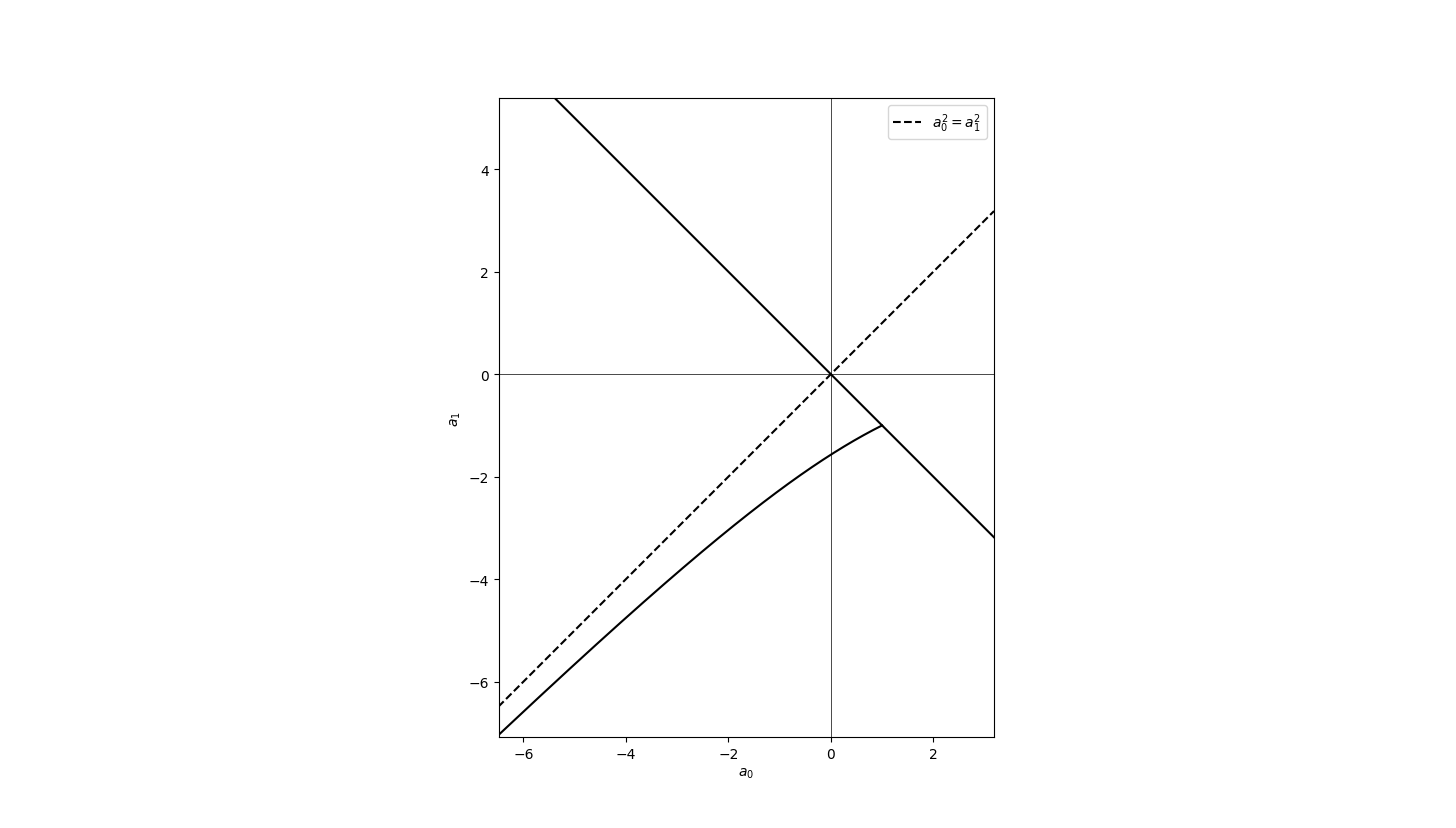
\includegraphics[width=\textwidth]{first-case}
  \caption{Граница $D$-разбиения}\label{fig:first-case}
\end{figure}

Так как матрица невырожденная, то константы $C_1, C_2$
определяются однозначно:
\begin{equation*}
  \begin{aligned}
    C_1
    &=
      \frac{\Delta_1}{\Delta}
      =
      -\frac{1}{4}
      \begin{vmatrix}
        0 & \dfrac{a_0}{a_1} + 1 \\
        -W & a_0 + a_1
      \end{vmatrix}
      =
      - \frac{W}{2}, \\
    C_2
    &=
      \frac{\Delta_2}{\Delta}
      =
      - \frac{1}{4}
      \begin{vmatrix}
        h - \dfrac{1}{a_1} & 0 \\
        a_1 h + 1 & -W
      \end{vmatrix}
      =
      \frac{a_1 h - 1}{4 a_1} W.
  \end{aligned}
\end{equation*}
Значит, решение вспомогательной системы равно
\begin{equation*}
  \begin{aligned}
    Y(\tau)
    &=
      -\frac{W}{2} \tau + \frac{a_1 h - 1}{4 a_1} W, \\
    Z(\tau)
    &=
      \frac{W}{2} \tau
      - \frac{W}{2 a_1}
      - \frac{a_1 h - 1}{4 a_1} W = \\
    &=
      \frac{W}{2} \tau
      - \frac{a_1 h + 1}{4 a_1} W.
  \end{aligned}
\end{equation*}

Так как константы $C_1, C_2$ определяются однозначно, то матрица
Ляпунова принимает вид~\cite[стр.~49]{kharitonov2013}
\begin{equation*}
  U(\tau) = Y(\tau)
  = - \frac{W}{2} \tau + \frac{a_1 h - 1}{4 a_1} W,
  \qquad \tau \in [0, h].
\end{equation*}

Подставим найденную матрицу Ляпунова в первое необходимое
условие~\eqref{eq:fredholm-2}; тогда
\begin{equation*}
  \begin{aligned}
    K(\theta, t)
    &=
      \begin{cases}
      \end{cases}
  \end{aligned}
\end{equation*}

\begin{equation*}
  K(\theta, t)
  =
  \frac{U(\theta - t)}{W_1 + (\theta + h) W_2},
  \qquad
  f(\theta)
  =
  - a_1 \varphi_0
  \frac{U(\theta + h)}{W_1 + (\theta + h) W_2},
  \qquad
  \lambda = -a_1^2.
\end{equation*}

\newpage
\subsection{Случай $a_0^2 > a_1^2$}

В этом случае характеристическое уравнение~\eqref{eq:aux-char}
имеет два вещественных корня
\begin{equation*}
  \lambda_1 = - \sqrt{ a_0^2 - a_1^2 },
  \qquad
  \lambda_2 = \sqrt{ a_0^2 - a_1^2 }.
\end{equation*}
Заметим, что $a_0 \neq 0$. Решение исходного
уравнения~\eqref{eq:aux-eq} представляется в виде
\begin{equation*}
  Y = C_1 e^{\lambda_1 \tau} + C_2 e^{\lambda_2 \tau}.
\end{equation*}
Найдём $Z(\tau)$. Для этого продифференцируем выражение для $Y$
и подставим в первое уравнение системы~\eqref{eq:aux-system}.
Имеем
\begin{equation*}
  \frac{d Y}{d \tau}
  = \lambda_1 C_1 e^{\lambda_1 \tau}
  + \lambda_2 C_2 e^{\lambda_2 \tau},
\end{equation*}
поэтому
\begin{equation*}
  \begin{aligned}
    Z
    &=
      \frac{1}{a_1} \frac{d Y}{d \tau} - \frac{a_0}{a_1} Y = \\
    &=
      \frac{1}{a_1} \left(
      \lambda_1 C_1 e^{\lambda_1 \tau}
      + \lambda_2 C_2 e^{\lambda_2 \tau}
      \right)
      - \frac{a_0}{a_1} \left(
      C_1 e^{\lambda_1 \tau} + C_2 e^{\lambda_2 \tau}
      \right) = \\
    &=
      \frac{\lambda_1 - a_0}{a_1} C_1 e^{\lambda_1 \tau}
      +
      \frac{\lambda_2 - a_0}{a_1} C_2 e^{\lambda_2 \tau}.
  \end{aligned}
\end{equation*}

Итак, решение вспомогательной системы~\eqref{eq:aux-system}
имеет вид
\begin{equation}
  \label{eq:aux-system-gen-solution}
  \begin{aligned}
    Y(\tau) &= C_1 e^{\lambda_1 \tau} + C_2 e^{\lambda_2 \tau}, \\
    Z(\tau) &=
              \frac{\lambda_1 - a_0}{a_1} C_1 e^{\lambda_1 \tau}
              +
              \frac{\lambda_2 - a_0}{a_1} C_2 e^{\lambda_2 \tau}.
  \end{aligned}
\end{equation}

Удовлетворим теперь граничным условиям~\eqref{eq:aux-boundaries}.
Подставим в них полученные представления для $Y$ и $Z$. Из
первого условия $Y(0) = Z(h)$ следует, что
\begin{equation*}
  C_1 + C_2 =
  \frac{\lambda_1 - a_0}{a_1} C_1 e^{\lambda_1 h}
  +
  \frac{\lambda_2 - a_0}{a_1} C_2 e^{\lambda_2 h}.
\end{equation*}
Из второго $2 a_0 Y(0) + a_1 Y(h) + a_1 Z(0) = -W$:
\begin{equation*}
  2 a_0 (C_1 + C_2) + a_1 \left(
    C_1 e^{\lambda_1 h} + C_2 e^{\lambda_2 h}
  \right)
  +
  (\lambda_1 - a_0) C_1 + (\lambda_2 - a_0) C_2 = -W.
\end{equation*}

После упрощений приходим к следующей системе:
\begin{equation}
  \begin{aligned}
    \left( 1 - \frac{\lambda_1 - a_0}{a_1} e^{\lambda_1 h} \right) C_1
    +
    \left( 1 - \frac{\lambda_2 - a_0}{a_1} e^{\lambda_2 h} \right) C_2 &= 0, \\
    \left(
    a_0 + a_1 e^{\lambda_1 h} + \lambda_1
    \right) C_1
    +
    \left(
    a_0 + a_1 e^{\lambda_2 h} + \lambda_2
    \right) C_2
    &= -W.
  \end{aligned}
\end{equation}

Найдём определитель этой системы:
\[
  \begin{aligned}
    \Delta
    &=
      \left( 1 - \frac{\lambda_1 - a_0}{a_1} e^{\lambda_1 h} \right)
      \cdot
      \left(
      a_0 + a_1 e^{\lambda_2 h} + \lambda_2
      \right)
      -
      \left( 1 - \frac{\lambda_2 - a_0}{a_1} e^{\lambda_2 h} \right)
      \cdot
      \left(
      a_0 + a_1 e^{\lambda_1 h} + \lambda_1
      \right) = \\
    &=
    \frac{e^{(h \lambda_1)} (a_0)^2}{a_1}
    - \frac{e^{(h \lambda_1)} a_0 \lambda_1}{a_1}
    + e^{(h \lambda_2)} a_1 - e^{(h \lambda_1 + h \lambda_2)} \lambda_1 + \\
    &\phantom{=}
    + \lambda_2 + \frac{e^{(h \lambda_1)} a_0 \lambda_2}{a_1}
    - \frac{e^{(h \lambda_1)} \lambda_1 \lambda_2}{a_1}
    + \frac{e^{(h \lambda_2)} a_0 \lambda_2}{a_1}
    - \frac{e^{(h \lambda_2)} (a_0)^2}{a_1} + \\
    &\phantom{=}
    + e^{(h \lambda_1 + h \lambda_2)} \lambda_2 - e^{(h \lambda_1)} a_1
    + \frac{e^{(h \lambda_2)} \lambda_1 \lambda_2}{a_1}
    - \frac{e^{(h \lambda_2)} a_0 \lambda_1}{a_1} - \lambda_1.
  \end{aligned}
\]
Так как $\lambda_2 = - \lambda_1$, то
\[
  \begin{aligned}
    \Delta
    &=
      \frac{e^{(h \lambda_1)} (a_0)^2}{a_1}
      - \frac{e^{(h \lambda_1)} a_0 \lambda_1}{a_1}
      + e^{(- h \lambda_1)} a_1
      - e^{(h \lambda_1 - h \lambda_1)} \lambda_1 + \\
    &\phantom{=}
      - \lambda_1 - \frac{e^{(h \lambda_1)} a_0 \lambda_1}{a_1}
      + \frac{e^{(h \lambda_1)} \lambda_1 \lambda_1}{a_1}
      - \frac{e^{(- h \lambda_1)} a_0 \lambda_1}{a_1}
      - \frac{e^{(- h \lambda_1)} (a_0)^2}{a_1} + \\
    &\phantom{=}
      - e^{(h \lambda_1 - h \lambda_1)} \lambda_1
      - e^{(h \lambda_1)} a_1
      - \frac{e^{(- h \lambda_1)} \lambda_1 \lambda_1}{a_1}
      - \frac{e^{(- h \lambda_1)} a_0 \lambda_1}{a_1}
      - \lambda_1 = \\
    &=
      \frac{e^{(h \lambda_1)} (a_0)^2}{a_1}
      + \frac{a_1}{e^{(h \lambda_1)}}
      - \frac{2 e^{(h \lambda_1)} a_0 \lambda_1}{a_1}
      + \frac{e^{(h \lambda_1)} (\lambda_1)^2}{a_1} - \\
    &\phantom{=}
      - \frac{(a_0)^2}{e^{(h \lambda_1)} a_1}
      - e^{(h \lambda_1)} a_1
      - \frac{(\lambda_1)^2}{e^{(h \lambda_1)} a_1}
      - \frac{2 a_0 \lambda_1}{e^{(h \lambda_1)} a_1}
      - 4 \lambda_1 = \\
    &=
      \frac{a_0^2}{a_1} \left(
      e^{h \lambda_1} - e^{-h \lambda_1}
      \right)
      - a_1 \left(
      e^{h \lambda_1} - e^{-h \lambda_1}
      \right)
      + \frac{\lambda_1^2}{a_1} \left(
      e^{h \lambda_1} - e^{-h \lambda_1}
      \right) - \\
    &\phantom{=}
      - \frac{2 a_0 \lambda_1}{a_1} \left(
      e^{h \lambda_1} - e^{-h \lambda_1}
      \right)
      - 4 \lambda_1 = \\
    &=
      2 \frac{\lambda_1^2}{a_1} \left(
      e^{h \lambda_1} - e^{-h \lambda_1}
      \right)
      - \frac{2 a_0 \lambda_1}{a_1} \left(
      e^{h \lambda_1} - e^{-h \lambda_1}
      \right)
      - 4 \lambda_1 = \\
    &=
      \frac{\lambda_1^2 - a_0 \lambda_1}{a_1}
      \sh (h \lambda_1)
      - 4 \lambda_1 = \\
    &= \lambda_1 \left[
      \frac{\lambda_1 - a_0}{a_1}
      \sh (h \lambda_1)
      - 4
      \right] = \\
    &= -\lambda_1 \left[
      \frac{\lambda_2 + a_0}{a_1}
      \sh (h \lambda_2)
      + 4
      \right].
  \end{aligned}
\]
Выясним, когда определитель равен нулю: $\Delta = 0$.
Так как $-\lambda_1 > 0$ и $\sh (h \lambda_2) > 0$, то
равенство нулю может достигаться только при
\[
  \frac{\lambda_2 + a_0}{a_1} < 0.
\]
Так как
\begin{equation*}
  \lambda_2 = \sqrt{a_0^2 - a_1^2} < \abs{a_0},
\end{equation*}
то знак числителя совпадает со знаком $a_0$. Таким образом,
определитель может равняться нулю только тогда, когда
$a_0$ и $a_1$ разных знаков.

Теорема 2.8 говорит о том, что в нашем случае
граничные условия будут однозначно определять решение
вспомогательной системы, поэтому кажется, что надо
просто принять, что $\Delta \neq 0$.

\subsection{Случай $a_0^2 < a_1^2$}

В этом случае характеристическое уравнение~\eqref{eq:aux-char}
имеет пару сопряжённых комплексных корней:
\begin{equation*}
  \lambda_1 = -i \sqrt{a_1^2 - a_0^2},
  \qquad
  \lambda_2 = i \sqrt{a_1^2 - a_0^2}.
\end{equation*}
Введём обозначение:
\begin{equation*}
  \lambda = \sqrt{a_1^2 - a_0^2}.
\end{equation*}
Решение исходного уравнения~\eqref{eq:aux-eq} представляется в
виде
\begin{equation*}
  Y = C_1 \cos \lambda \tau + C_2 \sin \lambda \tau.
\end{equation*}
Найдём $Z(\tau)$. Для этого продифференцируем выражение для $Y$
и подставим в первое уравнение системы~\eqref{eq:aux-system}.
Имеем
\begin{equation*}
  \frac{d Y}{d \tau}
  = - \lambda C_1 \sin \lambda \tau
  + \lambda C_2 \cos \lambda \tau.
\end{equation*}
поэтому
\begin{equation*}
  \begin{aligned}
    Z
    &=
      \frac{1}{a_1} \frac{d Y}{d \tau} - \frac{a_0}{a_1} Y = \\
    &=
      \frac{1}{a_1} \left(
      - \lambda C_1 \sin \lambda \tau
      + \lambda C_2 \cos \lambda \tau
      \right)
      - \frac{a_0}{a_1} \left(
      C_1 \cos \lambda \tau + C_2 \sin \lambda \tau
      \right) = \\
    &=
      - \frac{\lambda C_1}{a_1} \sin \lambda \tau
      + \frac{\lambda C_2}{a_1} \cos \lambda \tau
      - \frac{a_0 C_1}{a_1} \cos \lambda \tau
      - \frac{a_0 C_2}{a_1} \sin \lambda \tau = \\
    &=
      \frac{\lambda C_2 - a_0 C_1}{a_1}
      \cos \lambda \tau
      -
      \frac{\lambda C_1 + a_0 C_2}{a_1}
      \sin \lambda \tau.
  \end{aligned}
\end{equation*}

Итак, решение вспомогательной системы~\eqref{eq:aux-system}
имеет вид
\begin{equation}
  \label{eq:aux-system-gen-solution}
  \begin{aligned}
    Y(\tau)
    &=
      C_1 \cos \lambda \tau + C_2 \sin \lambda \tau, \\
    Z(\tau)
    &=
      \frac{\lambda C_2 - a_0 C_1}{a_1}
      \cos \lambda \tau
      -
      \frac{\lambda C_1 + a_0 C_2}{a_1}
      \sin \lambda \tau.
  \end{aligned}
\end{equation}

Удовлетворим теперь граничным условиям~\eqref{eq:aux-boundaries}.
Подставим в них полученные представления для $Y$ и $Z$. Из
первого условия $Y(0) = Z(h)$ следует, что
\begin{equation*}
  C_1
  =
  \frac{\lambda C_2 - a_0 C_1}{a_1}
  \cos \lambda h
  -
  \frac{\lambda C_1 + a_0 C_2}{a_1}
  \sin \lambda h.
\end{equation*}
Из второго $2 a_0 Y(0) + a_1 Y(h) + a_1 Z(0) = -W$:
\begin{equation*}
  2 a_0 C_1
  + a_1 \left(
    C_1 \cos \lambda h + C_2 \sin \lambda h
  \right)
  + \lambda C_2 - a_0 C_1 = -W.
\end{equation*}
После упрощений получаем систему
\begin{equation*}
  \begin{aligned}
    \left(
    \frac{\lambda \sin \lambda h}{a_1}
    + \frac{a_0 \cos \lambda h}{a_1}
    + 1
    \right)
    C_1
    +
    \left(
    \frac{a_0 \sin \lambda h}{a_1}
    - \frac{\lambda \cos \lambda h}{a_1}
    \right)
    C_2
    &= 0, \\
    \left(
    a_0 + a_1 \cos \lambda h
    \right)
    C_1
    +
    \left(
    a_1 \sin \lambda h + \lambda
    \right)
    C_2
    &=
      -W.
  \end{aligned}
\end{equation*}
Найдём её определитель:
\begin{equation*}
  \begin{aligned}
    \Delta
    &=
      \left(
      \frac{\lambda \sin \lambda h}{a_1}
      + \frac{a_0 \cos \lambda h}{a_1}
      + 1
      \right)
      \left(
      a_1 \sin \lambda h + \lambda
      \right)
      -
      \left(
      \frac{a_0 \sin \lambda h}{a_1}
      - \frac{\lambda \cos \lambda h}{a_1}
      \right)
      \left(
      a_0 + a_1 \cos \lambda h
      \right)
      = \\
    &=
      \lambda \sin^2 \lambda h + a_1 \sin \lambda h
      + \frac{\lambda^2 \sin \lambda h}{a_1} + \lambda
      + \frac{2 \lambda a_0 \cos \lambda h}{a_1}
      - \frac{a_0^2 \sin \lambda h}{a_1}
      + \lambda \cos^2 \lambda h = \\
    &=
      2 \lambda
      + \frac{a_1^2 \sin \lambda h}{a_1}
      + \frac{
      a_1^2 \sin \lambda h - a_0^2 \sin \lambda h
      - a_0^2 \sin \lambda h
      }{a_1}
      + \frac{2 \lambda a_0 \cos \lambda h}{a_1} = \\
    &=
      2 \lambda
      + \frac{2 \lambda^2 \sin \lambda h}{a_1}
      + \frac{2 \lambda a_0 \cos \lambda h}{a_1} = \\
    &=
      \frac{2 \lambda}{a_1} \left(
      a_1 + \lambda \sin \lambda h + a_0 \cos \lambda h
      \right).
  \end{aligned}
\end{equation*}
Тогда
\begin{equation*}
  \begin{aligned}
    C_1
    &=
      \frac{\Delta_1}{\Delta}
      =
      \frac{1}{\Delta}
      \begin{vmatrix}
        0 & \dfrac{
            a_0 \sin \lambda h - \lambda \cos \lambda h
            }{a_1} \\
        -W & a_1 \sin \lambda h + \lambda
      \end{vmatrix}
      = \\
    &=
      \frac{
      W \left(
      a_0 \sin \lambda h - \lambda \cos \lambda h
      \right)
      }{
      2 \lambda \left(
      a_1 + \lambda \sin \lambda h + a_0 \cos \lambda h
      \right)
      }, \\
    C_2
    &=
      \frac{\Delta_2}{\Delta}
      =
      \frac{1}{\Delta}
      \begin{vmatrix}
        \dfrac{
        \lambda \sin \lambda h
        + a_0 \cos \lambda h
        + a_1
        }{a_1} & 0 \\
        a_0 + a_1 \cos \lambda h & -W
      \end{vmatrix}
      = \\
    &=
      -\frac{W \left(
        \lambda \sin \lambda h
        + a_0 \cos \lambda h
        + a_1
      \right)}{
      2 \lambda \left(
        \lambda \sin \lambda h
        + a_0 \cos \lambda h
        + a_1
      \right)
      }
      = \\
    &= -\frac{W}{2 \lambda}.
  \end{aligned}
\end{equation*}
Значит, матрица Ляпунова имеет вид
\begin{equation*}
  U(\tau) = Y(\tau)
  =
  \frac{
    W \left(
      a_0 \sin \lambda h - \lambda \cos \lambda h
    \right)
  }{
    2 \lambda \left(
      a_1 + \lambda \sin \lambda h + a_0 \cos \lambda h
    \right)
  } \cos \lambda \tau
  - \frac{W}{2 \lambda} \sin \lambda \tau.
\end{equation*}

% \newpage

% \appendix

% \section{Приложение}

% \subsection{Таблица интегралов}

\newpage

\addcontentsline{toc}{section}{Список использованных источников}
\renewcommand{\refname}{Список использованных источников}
\begin{center}
  \nocite{gelfand1961}
  \printbibliography{}
\end{center}

\end{document}
